\documentclass[20pt]{extarticle}

\usepackage[paperwidth=841mm,paperheight=1189mm,margin=20mm]{geometry}
\usepackage{lmodern}
\usepackage{graphicx}
\usepackage[table]{xcolor}
\usepackage{booktabs}
\usepackage{tabularx}
\usepackage{array}
\usepackage{enumitem}
\usepackage{amsmath}
\usepackage{qrcode}
\usepackage{hyperref}
\usepackage{ragged2e}

\pagestyle{empty}
\setlength{\parindent}{0pt}
\setlength{\parskip}{3mm}
\renewcommand{\familydefault}{\rmdefault}
\urlstyle{same}

\definecolor{Night}{HTML}{071017}
\definecolor{Panel}{HTML}{0D1A23}
\definecolor{Paper}{HTML}{F1F0E8}
\definecolor{Muted}{HTML}{B8C3C8}
\definecolor{Rule}{HTML}{3B515E}
\definecolor{Cyan}{HTML}{56B4E9}
\definecolor{Orange}{HTML}{E69F00}
\definecolor{Magenta}{HTML}{CC79A7}
\definecolor{Lime}{HTML}{B8E038}
\definecolor{Coral}{HTML}{E76F51}
\pagecolor{Night}
\color{Paper}

\hypersetup{
  colorlinks=false,
  pdfborder={0 0 0},
  pdftitle={The Perturbation Catalogue: An Integrated Resource for Exploring the Impact of Genetic Perturbations},
  pdfauthor={Kirill Tsukanov, Aleksandr Zakirov, Alexey Sokolov, Mallory Freeberg}
}

\newcommand{\sectiontitle}[2]{%
  \vspace{4mm}%
  {\color{#1}\rule{\linewidth}{1.6mm}}\par\vspace{2mm}%
  {\fontsize{39}{43}\selectfont\bfseries #2}\par\vspace{3mm}}

\newcommand{\subsectiontitle}[2]{%
  {\fontsize{26}{30}\selectfont\bfseries\color{#1}#2}\par\vspace{1mm}}

\newcommand{\bodycopy}{\fontsize{24}{30}\selectfont}
\newcommand{\smallcopy}{\fontsize{20}{25}\selectfont}
\newcommand{\metric}[2]{%
  {\fontsize{31}{34}\selectfont\bfseries\color{#1}#2}}

\newcolumntype{Y}{>{\RaggedRight\arraybackslash}X}
\newcolumntype{L}[1]{>{\RaggedRight\arraybackslash}p{#1}}

\begin{document}

% Title -----------------------------------------------------------------------
{\color{Lime}\rule{18mm}{4mm}}\hspace{5mm}
{\fontsize{18}{21}\selectfont\bfseries\color{Muted}EMBL European Bioinformatics Institute}

\vspace{6mm}
{\fontsize{58}{63}\selectfont\bfseries
The Perturbation Catalogue:\\[-1mm]
{\fontsize{43}{48}\selectfont An Integrated Resource for Exploring the Impact of Genetic Perturbations}\par}

\vspace{5mm}
{\fontsize{21}{26}\selectfont
Kirill Tsukanov \textbullet\ Aleksandr Zakirov \textbullet\ Alexey Sokolov \textbullet\ Mallory Freeberg\\
\color{Muted}EMBL European Bioinformatics Institute, Wellcome Genome Campus, Hinxton, United Kingdom}

\vspace{5mm}
\noindent
\begin{minipage}[t]{0.73\linewidth}
  {\fontsize{27}{34}\selectfont
  Large-scale perturbation studies reveal gene function, disease mechanisms and candidate drug targets,
  but their evidence remains fragmented across repositories, formats, identifiers and study-specific processing choices.
  The Perturbation Catalogue brings these experiments into a shared, searchable resource while retaining the biological
  and technical context needed to interpret every result.}
\end{minipage}\hfill
\begin{minipage}[t]{0.23\linewidth}
  {\color{Rule}\rule{1.8mm}{48mm}}\hspace{5mm}
  \begin{minipage}[t]{0.82\linewidth}
    {\fontsize{25}{31}\selectfont\bfseries\color{Lime}Three complementary scales of evidence}\par
    \vspace{3mm}{\smallcopy
    For a target of interest, the Catalogue links \textcolor{Orange}{gene-level screening phenotypes},
    \textcolor{Magenta}{variant-level functional measurements} and
    \textcolor{Cyan}{single-cell transcriptomic responses}.}
  \end{minipage}
\end{minipage}

\vspace{6mm}

% Modality matrix -------------------------------------------------------------
\sectiontitle{Cyan}{What each modality contributes}
{\smallcopy
\renewcommand{\arraystretch}{1.45}
\setlength{\tabcolsep}{5mm}
\rowcolors{2}{Panel}{Night}
\begin{tabularx}{\linewidth}{L{123mm}YYY}
\toprule[1.2mm]
& \textbf{\color{Cyan}\Large Perturb-Seq}
& \textbf{\color{Orange}\Large CRISPR screens}
& \textbf{\color{Magenta}\Large MAVE}\\
\midrule[.6mm]
\textbf{Resolution} & Single cell; gene perturbation $\times$ transcriptome & Gene perturbation $\times$ phenotype or fitness & Amino-acid or nucleotide variant $\times$ functional score\\
\textbf{Primary readout} & Cell-by-gene expression counts & Gene-level depletion, enrichment or assay score & Variant effect measurements across protein sequence\\
\textbf{Catalogue analysis} & Standardised differential expression and Hallmark gene-set enrichment & Harmonised author-generated scores and significant hits & Harmonised author-generated scores and variant-effect heatmaps\\
\textbf{Explore by} & Perturbed target, affected gene, dataset and biological context & Perturbed target, dataset and biological context & Target, variant position, amino-acid change and dataset\\
\textbf{Current production coverage} & \textbf{26 datasets}; five reprocessed from raw FASTQ & \textbf{1,201 datasets} & \textbf{10 datasets}\\
\bottomrule[1.2mm]
\end{tabularx}}

\vspace{7mm}

% Three information-dense columns --------------------------------------------
\noindent
\begin{minipage}[t]{0.305\linewidth}
  \sectiontitle{Orange}{Why integration is difficult}
  {\bodycopy
  A published result is inseparable from its experimental design. The same perturbation can produce different effects
  across model systems, assay endpoints, delivery methods, time points and analysis pipelines. Gene symbols change;
  repositories expose different identifiers; metadata depth varies; and useful context is often available only in the paper
  or supplement.

  The Catalogue therefore preserves source provenance while converting data and metadata into common structures.
  The goal is not to erase genuine biological differences, but to remove avoidable friction before comparison and reuse.}

  \sectiontitle{Magenta}{Metadata that carries meaning}
  {\bodycopy
  Each curated dataset is validated against a unified, extensible schema. Core domains include:}

  \vspace{2mm}
  \subsectiontitle{Cyan}{Study}
  {\smallcopy Title, authors, accession, publication year, source repository and licence.}

  \subsectiontitle{Orange}{Perturbation}
  {\smallcopy Mechanism, library generation, enzyme and library delivery, treatment and time point.}

  \subsectiontitle{Magenta}{Assay}
  {\smallcopy Readout, sequencing platform, software, score interpretation and processing provenance.}

  \subsectiontitle{Lime}{Model system}
  {\smallcopy Tissue, cell type or cell line, disease, sex and developmental stage.}

  \subsectiontitle{Cyan}{Target}
  {\smallcopy Ensembl gene ID, approved symbol and name, biotype and genomic identity.}

  \vspace{3mm}
  {\bodycopy
  Biological entities are aligned to established ontologies wherever possible. Curation also reveals missing or inadequate
  terms, allowing the project to contribute improvements back to ontology communities.}

  \sectiontitle{Lime}{Production catalogue at a glance}
  \begin{tabularx}{\linewidth}{@{}Y Y@{}}
    \metric{Lime}{1,237} datasets & \metric{Cyan}{19,235} targets\\[3mm]
    \metric{Orange}{36} tissues & \metric{Magenta}{34} cell types\\[3mm]
    \metric{Cyan}{1,200} cell lines & \metric{Orange}{169} diseases
  \end{tabularx}
  {\fontsize{14}{17}\selectfont\color{Muted}Production snapshot: 24 August 2026.}
\end{minipage}
\hfill
\begin{minipage}[t]{0.355\linewidth}
  \sectiontitle{Cyan}{How evidence enters the Catalogue}
  {\bodycopy
  Public repositories and published studies are curated into modality-specific inputs, validated, normalised and transformed
  into shared analytical and metadata tables. The same backend and API then serve every modality.}

  \vspace{4mm}
  {\fontsize{19}{24}\selectfont
  \[
    \text{sources}
    \longrightarrow \underbrace{\text{curation + validation}}_{\text{shared schema}}
    \longrightarrow \underbrace{\text{BigQuery + dbt}}_{\text{harmonised tables}}
    \longrightarrow \underbrace{\text{Elastic + Postgres}}_{\text{search + data}}
    \longrightarrow \text{API / portal / files}
  \]}

  {\bodycopy
  Ensembl gene IDs provide the stable target identity across ingestion, search and retrieval. Dataset-level provenance,
  licence and score interpretation remain visible rather than being detached from the measurements they qualify.}

  \sectiontitle{Orange}{Perturb-Seq reprocessing from raw FASTQ}
  {\bodycopy
  Author-provided expression matrices differ in alignment software, gene annotation, filtering and guide assignment.
  Our reprocessing workflow starts again from raw sequencing reads so that selected studies share one computational path:}

  \vspace{3mm}
  {\fontsize{22}{27}\selectfont\bfseries\color{Paper}
  \[
  \mathrm{FASTQ}
  \rightarrow \mathrm{cell\!\times\!gene\ counts}
  \rightarrow \mathrm{guide\ assignment}
  \rightarrow \mathrm{QC}
  \rightarrow \mathrm{DEA}
  \rightarrow \mathrm{GSEA}
  \]}

  {\bodycopy
  Differential expression records the direction and magnitude of gene-level response to each perturbation. Gene-set
  enrichment summarises coordinated changes using MSigDB Hallmark pathways. Final data, summaries and provenance are
  published through the same Catalogue interface and API.}

  \vspace{2mm}
  {\fontsize{19}{24}\selectfont\bfseries\color{Lime}Five reprocessed datasets are live:}
  {\smallcopy
  \begin{itemize}[leftmargin=8mm,itemsep=1mm,topsep=2mm]
    \item Nadig 2025: Jurkat and HepG2
    \item Replogle 2022: K562 essential, K562 genome-wide and RPE1 essential
  \end{itemize}}

  \sectiontitle{Magenta}{What “comparable” means here}
  {\bodycopy
  Shared processing reduces avoidable technical variation; it does not make distinct experiments biologically equivalent.
  Current validation compares broad agreement with author-generated matrices where available. Developing author-independent
  quality metrics and wider kit support remains an active part of the work.}
\end{minipage}
\hfill
\begin{minipage}[t]{0.305\linewidth}
  \sectiontitle{Magenta}{Explore targets and datasets}
  {\bodycopy
  Search a gene once to see which modalities contain evidence, which datasets contribute it, significant perturbation effects
  and top enriched pathways. Dataset pages expose the full curated context and distinguish author-provided from reprocessed data.}

  \vspace{4mm}
  {\setlength{\fboxsep}{2mm}\fcolorbox{Rule}{Panel}{%
    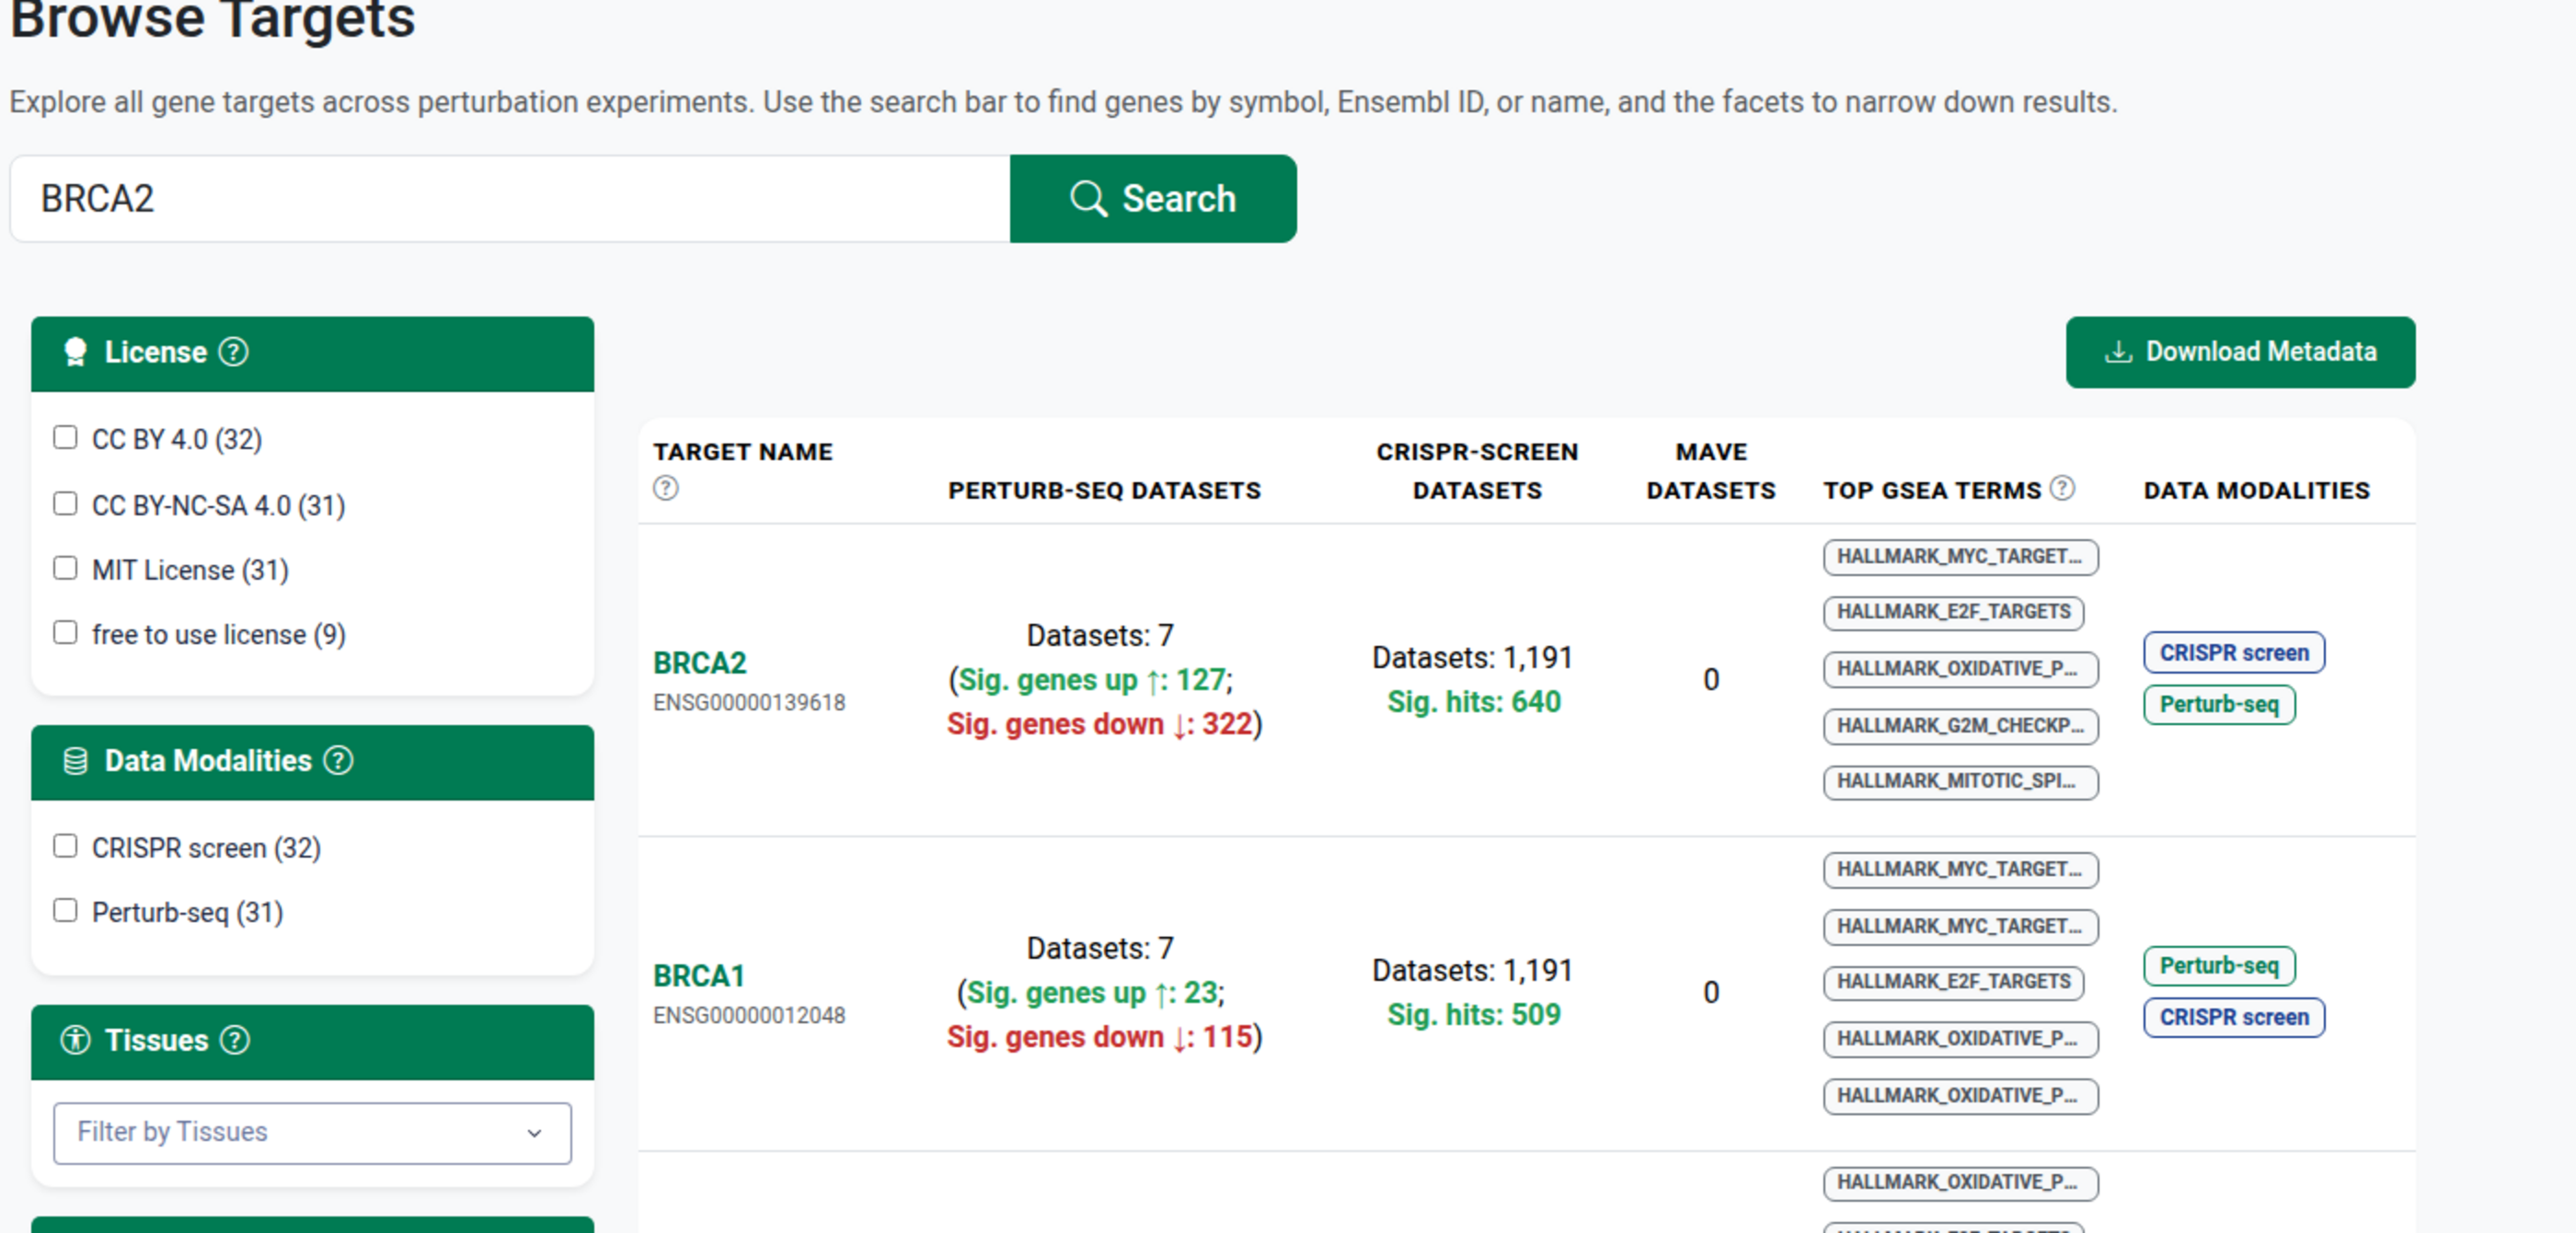
\includegraphics[width=0.97\linewidth]{assets/target-search.png}}}
  {\fontsize{15}{18}\selectfont\color{Muted}
  Live target browser for BRCA2: modality coverage, significant hits and Hallmark enrichment terms.}

  \sectiontitle{Cyan}{Available now}
  {\bodycopy
  \begin{itemize}[leftmargin=8mm,itemsep=2mm,topsep=0mm]
    \item Search and filter targets or datasets across all three modalities.
    \item Inspect curated experimental context, ontology links, licence and provenance.
    \item Explore Perturb-Seq differential expression and pathway enrichment.
    \item View significant CRISPR hits and MAVE variant-effect heatmaps.
    \item Use Ensembl gene IDs consistently across modalities.
  \end{itemize}}

  \sectiontitle{Orange}{API and complete downloads}
  {\bodycopy
  Everything displayed by the portal is available programmatically. Common entry points include:}

  \vspace{2mm}
  {\fontsize{15}{20}\selectfont\ttfamily\color{Lime}
  GET /search?query=BRCA2\&search\_mode=targets\\[2mm]
  GET /dataset/\{dataset\_id\}\\[2mm]
  GET /v1/perturb-seq/\{dataset\_id\}/search}

  \vspace{4mm}
  {\bodycopy
  Full datasets are precomputed as \textbf{Parquet} and gzip-compressed \textbf{CSV}; dataset metadata is available as
  \textbf{JSON}. Filtered table views can also be downloaded directly, making the Catalogue useful both interactively and
  inside reproducible workflows.}
\end{minipage}

\vspace{7mm}

% Concrete production example -------------------------------------------------
\sectiontitle{Lime}{Inside a reprocessed Perturb-Seq dataset}
\noindent
\begin{minipage}[t]{0.30\linewidth}
  \vspace{1mm}
  {\setlength{\fboxsep}{2mm}\fcolorbox{Rule}{Paper}{%
    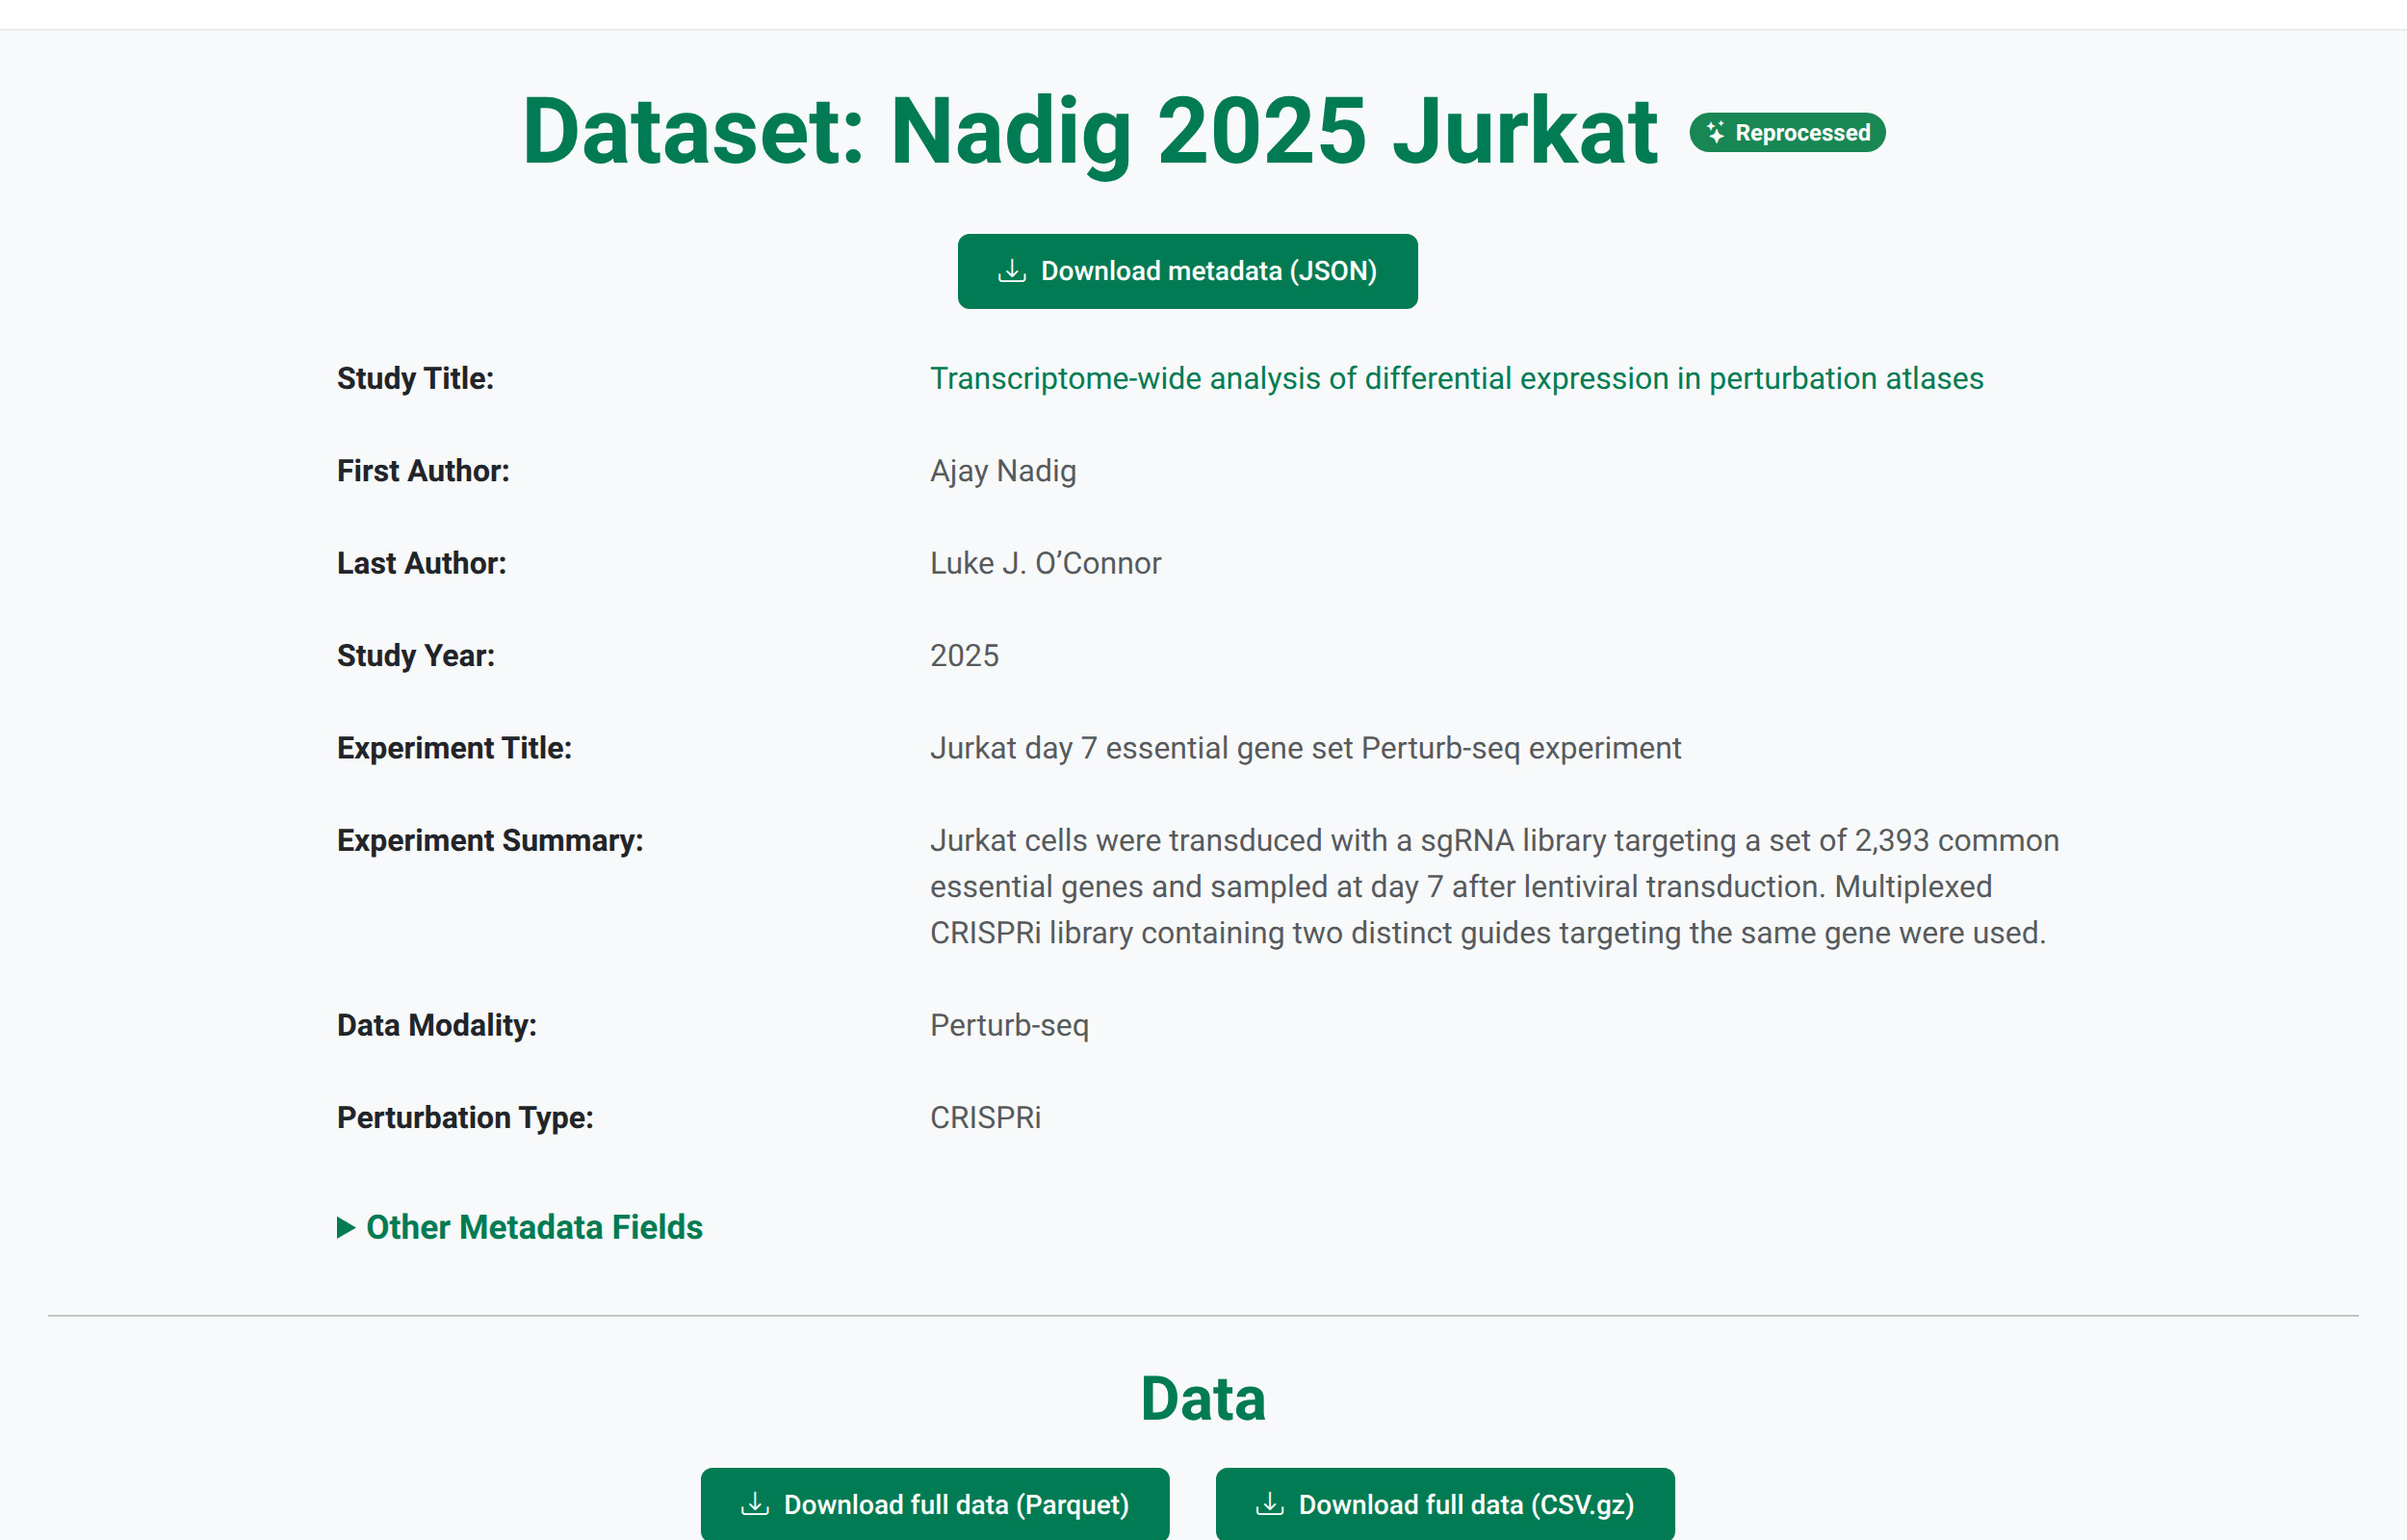
\includegraphics[width=0.975\linewidth]{assets/nadig-dataset.png}}}
\end{minipage}\hfill
\begin{minipage}[t]{0.66\linewidth}
  \subsectiontitle{Cyan}{Interpretation begins before the first result}
  {\bodycopy
  The dataset page identifies the source study, experiment, modality and perturbation mechanism, and labels data that have
  been reprocessed from raw sequencing reads. Additional metadata remains one click away rather than being reduced to a
  detached accession number.}

  \vspace{3mm}
  \subsectiontitle{Orange}{From summary to the complete evidence}
  {\bodycopy
  Interactive rows connect perturbations and effect genes to Ensembl IDs, effect size, adjusted significance, statistical
  score and biological context. The same page provides complete Parquet and compressed CSV files—not only the rows visible
  after filtering.}

  \vspace{3mm}
  \subsectiontitle{Magenta}{Metadata is data, too}
  {\bodycopy
  The full validated metadata record is downloadable as JSON. This makes experimental context and provenance available to
  computational workflows, supports reproducible reuse and exposes exactly how a dataset was interpreted by the Catalogue.}

  \vspace{3mm}
  {\smallcopy\color{Muted}
  Production example: Nadig 2025 Jurkat. The reanalysis targets 2,393 common essential genes in a day-7 CRISPRi experiment.}
\end{minipage}

\vspace{7mm}

% Roadmap, collaboration and single QR ---------------------------------------
{\color{Lime}\rule{\linewidth}{2.2mm}}\par\vspace{4mm}
\noindent
\begin{minipage}[t]{0.35\linewidth}
  {\fontsize{34}{38}\selectfont\bfseries What we are building next}\par\vspace{3mm}
  {\bodycopy
  Curator-reviewed metadata extraction; broader, modality-appropriate reanalysis; support for additional datasets and
  experimental designs; and periodic, versioned releases with explicit provenance.}
\end{minipage}\hfill
\begin{minipage}[t]{0.29\linewidth}
  {\fontsize{34}{38}\selectfont\bfseries Work with us}\par\vspace{3mm}
  {\bodycopy
  Suggest a dataset, challenge our schema or request a feature. Funded multi-year collaborations can prioritise the
  modalities, datasets, analyses or functionality most relevant to your programme.}

  {\fontsize{21}{25}\selectfont\bfseries\color{Lime}
  perturbation-catalogue-help@ebi.ac.uk}
\end{minipage}\hfill
\begin{minipage}[t]{0.18\linewidth}
  \centering
  {\fontsize{22}{25}\selectfont\bfseries Explore the Catalogue}\par\vspace{3mm}
  {\color{Paper}\href{https://www.ebi.ac.uk/perturbation-catalogue/}{\qrcode[height=58mm]{https://www.ebi.ac.uk/perturbation-catalogue/}}}
\end{minipage}\hfill
\begin{minipage}[t]{0.12\linewidth}
  \RaggedLeft
  
\includegraphics[width=80mm]{assets/embl-ebi-logo.png}\\[6mm]
  
\includegraphics[width=80mm]{assets/open-targets-logo.png}
\end{minipage}

\end{document}
